% chap2.tex - Woche 2
\chapter{Woche 2}
\section{Tag 1 - ``Wir sind Programmierer, wir benutzen Git!''}
\subsection{Die Entwicklungsumgebung aufsetzen}


Jetzt sind wir also bereit in die Tiefen von Git abzutauchen und es tats"achlich zu benutzen, oder? Naja, nicht wirklich. Zuerst m"ussen wir uns entscheiden, wie der Workflow, f"ur den wir uns entschieden haben, in unserem Versionsverwaltungssystem implementiert werden soll. Die Tatsache, dass Git so vielseitig ist, ist Segen und Fluch zugleich. Es ist eine gute Idee von Anfang an festzulegen, wie sich Entwickler, Reviewer und Integratoren verhalten sollen, bevor man tats"achlich anf"angt Code zu committen. Aber manchmal ist das nicht m"oglich. Es ist gut m"oglich, dass Du noch nie ein Versionskontrollsystem wie Git benutzt hast und Du daher anf"angst, Dich durch das Thema durchzuk"ampfen.  Das ist zwar normal, aber falls Du vor hast diese Art von System in eine produktive Umgebung einzupflegen, solltest Du erst herausfinden, wie das "uberhaupt funktioniert. 

Das Modell, welches vorhin vorgestellt wurde, ist leicht vorzustellen. Wir haben zwei Integratoren, die beide Zugriff auf das Blessed Repository haben, und es gibt mehrere Entwickler, deren Changes gereviewed und integriert werden; eben von jenen Integratoren. Die physische Darstellung dieses Workflow-Modells ist im Diagramm unten aufgef"uhrt.

\begin{figure}[bt]
\centering
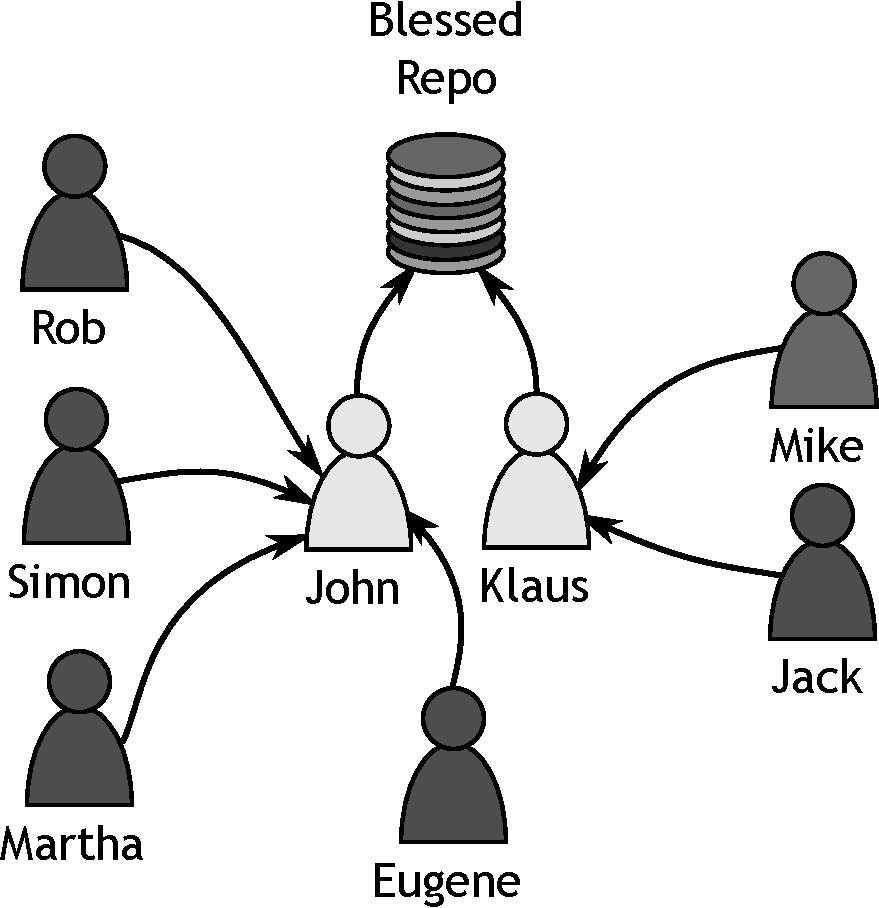
\includegraphics[width=7cm]{images/f-w2-d1.pdf}
\caption{Tamagoyaki Inc's Physical Structure}
\end{figure}

Die physische Struktur is einfach und gut, aber sie legt nicht genau fest, wie die Daten bewegt werden, sie legt lediglich fest, wer daf"ur verantwortlich ist auf der jeweilgigen Stufe des Ablaufs. Was nun ben"otigt wird, ist eine detaillierte Analyse wo die Daten herkommen und wo sie sich hinbewegen. Ein Datenflussdiagramm ist hierf"ur n"utzlich, aber nicht essentiell. Nichtsdestotrotz werden wir eine leicht ver"anderte Form des Diagrammes, um zeigen zu k"onnen, wie die Daten von einer Person zur anderen "ubertragen werden. Bevor wir fortfahren und einen Blick auf das Diagramm werfen, lass uns kurz in die Sch"utzengr"aben zur"uckkehren und nachschauen, wie die Leute mit ihrem Repository-Design zurechtkommen.

\begin{trenches}
``John, warum muessen wir uns an einem Montag Morgen um 09:45 Uhr hier treffen.'' beklagte sich Klaus. ``Ich habe noch nicht einmal genug Kaffee intus, um meine E-Mails zu checken, ganz zu schweigen von einem Meeting!''

John grinste, ``Ich glaube nicht, dass Dir Kaffee da helfen w"urde, Klaus. Es ist eine Gewinner-Pers"onlichkeit, die Dir da helfen wird.'' Der Rest des Teams lachte, bis John begann wild auf dem Whiteboard zu zeichnen. ``Also, hier haben wir unser phsyisches Modell. Wir wissen, welche Leute die Verantwortung tragen werden, aber wir wissen nicht, wie wir unsere Repositories anordnen sollen.''

``Guter Einwand,'' stimme Mike ihm zu.

``Also, wir werden offenbar ein Blessed Repository haben,'' sagte John, w"ahrend er einen Kreis auf die Tafel malte. Er trat zur"uck, eine Hand am Kinn. ``Weiterhin stelle ich mir vor, dass Klaus und Ich Kopien dieses Repositories auf unseren lokalen Festplatten haben. Wir werden diese modifizieren und dann unsere Changes zur"uck in das zentrale Repository schieben.''

``Aber ich dachte Git hat kein zentrales Repository?'' fragte Martha. Die anderen st"ohnten.

``Nun,'' sagte John, ``so weit ich das verstanden habe, hat es das tats"achlich nicht. Was ich meine, ist, dass Klaus und Ich auch lokale Kopien des Repositories haben. Wir arbeiten an diesen lokalen Kopien und pushen unsere Ver"anderungen zur"uck auf den Server. Es ist eine Synchronisation, und auch eine Kopie. Ich glaube, das nennt man einen Klon.'' Er nickte, ``Und da Klaus und ich kaum am selben Code arbeiten, m"ussen wir wohl kaum mergen oder mit Konflikten rechnen.''

``Aber was ist mit uns Codeaffen?'' fragte Martha, ``Woher koennen wir unsere Kopien des Repositories beziehen?''

``Vom zentralen Server nat"urlich,'' Rob begann zu l"acheln.

``Ja,'' sagte John, ``aber Ich denke, was Martha sagen will ist, wie Ihr die Updates bekommen werdet?'' Er begann im Raum herumzulaufen und der eine oder andere der Entwickler folgte ihm, als er das Fenster erreichte und stehen blieb. ``Ich denke Ihr w"urdet Euren Branch mit dem des Blessed Repositories mergen.''

Im Zimmer wurde es still und das einzige Ger"ausch das zu h"oren war, war das rattern der Klimaanlahe in der Zimmerdecke.

Simon fing an zu rede, ``Naja, ich habe am Wochenende etwas "uber dieses Rebasing gelesen und in manchen F"allen soll ein Rebase besser als Merging sein.''

``Was ist Rebasing und worin unterscheidet es sich zum Merging?'' fragte Mike.

Nun, Rebasing ist ziemlich clever. Stell Dir das folgendermassen vor: Du hast einen Upstream Branch, in unserem Fall das Blessed Repository. Du machst Changes. Wenn sich der Upstream Branch "andert k"onntest Du die Changes vom Blessed Repository reinmergen. Wenn Du das machst erstellst Du einen eigenen Commit hierf"ur, der die Ver"anderungen merged. Das funktioniert zwar, aber\ldots'' er driftete ein wenig ab, ``es kann unter Umst"anden Probleme verursachen. Ein besserer Weg das zu handhaben ist Rebasing. Rebasing kann alle Ver"anderungen, die Du gemacht hast nehmen, sie auf die Seite r"aumen und alle Upstream-Changes einf"ugen. Danach werden die vorher beseitigten Changes auf die gerade eingef"ugten Changes draufgesetzt.''

John atmete aus, ``Das klingt ziemlich cool Simon, aber eine Sache ist glasklar, wir m"ussen mehr "uber die Grundlagen von Git lernen, bevor wir anfangen uns mit Merging und Rebasing zu besch"aftigen. Lasst uns den Rest des Tages damit verbringen, mit einigen Test-Repositories zu experimentieren und morgen treffen wir uns dann wieder.''
\end{trenches}

Falls Du noch nie zuvor mit einem VCS zu tun hattest, ist es eine gute Idee, zuvor einige Zeit lang damit herumzuspielen. Schon sehr bald wirst Du die Grundlagen gelernt haben und in der Lage sein, Deine neu erworbenen F"ahigkeiten in die Praxis umzusetzen. Aber obwohl es gut ist, in Test-Repositories zu experimentieren, ist es ganz normal, dass man das System tats"achlich benutzen muss um Probleme zu entdecken. Der Rest dieses Kapitels ist eine sehr kurze Einf"uhrung in Git. Es ist aufgebaut wie eine Einf"uhrung, weil wir erwarten, dass Du Dir etwas Zeit nimmst um Git kennenzulernen und zu lernen wie es funktioniert.

\subsection{Ein Repository initialisieren}
Das erste, das wir machen m"ussen, ist zwei sehr wichtige Sachen verstehen:

\begin{enumerate}
  \item Wie man ein Git Repository erstellt
  \item Was ein Git Repository tats"achlich ist
\end{enumerate}

Das erste davon ist relativ einfach umzusetzen.

\begin{Verbatim}
john@satsuki:~$ mkdir coderepo
john@satsuki:~$ cd coderepo/
john@satsuki:~/coderepo$ git init
Initialized empty Git repository in /home/john/coderepo/.git/
john@satsuki:~/coderepo$
\end{Verbatim}

Was wir hier gemacht haben, ist folgendes: Wir haben ein neues Verzeichnis namens coderepo erstellt, in dieses Verzeichnis gewechselt und das Kommando git init aufgerufen. Das Resultat dieses Aufrufs ist ein neues Verzeichnis im coderepo-Ordner, das .git hei"st. Dieses Verzeichnis beinhaltet eine lokale Kopie unseres kompletten Repositories. Es erm"oglicht uns die Erstellung von Branches, das Mergen von Changes, Rebasing und letzten Endes auch das Pushen von unseren Changes auf einen Server.

Etwas, das sehr wichtig beim Betreiben eines Repositories ist, sowohl f"ur Git-Administratoren als auch Entwickler die es benutzen, das Verst"andnis wie Git funktioniert. Es ist sch"on ins kalte Wasser zu springen und durch Experimente das Wasser zu testen, aber bevor man sich verpflichtet Git in einer produktiven Umgebung zu benutzen, sollte man verstehen, was Git im Hintergrund macht.

W"ahrend Ich dieses Buch geschrieben habe, haben mir verschiedene Leute erz"ahlt, dass Git eines der wenigen VCS ist, wo ein gutes Verst"andnis des zugrunde liegenden Systems nicht nur hilfreich, sondern sogar beinahe n"otig ist.

Nehmen wir uns ein paar Minuten Zeit um dar"uber zu reden, wie Git intern funktioniert und wie die Daten tats"achlich gespeichert werden. Git speichert Changes nicht in Dateien, sondern Snapshots zu bestimmten Zeitpunkten. Es bezieht sich auf diese, indem es einen SHA-1 Hash gegen sie vergleicht. Dadurch ist es f"ur Git einfach zu erkennen, ob eine Datei ver"andert wurde. Wenn sich ein SHA-1 Hash einer Datei "andert hat sich der Inhalt der Datei offensichtlich ver"andert.

Wenn ein Commit im Repository gemacht wird, speichert Git einige Dinge: Ein Commit Object wird erstellt, welches Informationen dar"uber enth"alt, wer den Commit gemacht hat, den Ursprung des Commits und ein Tree Object. Das Tree Object beschreibt, wie das Repository zum Zeitpunkt des Commits ausgesehen hat. In anderen Worten: Der Tree Object teilt Git mit, welche Dateien im Repository enthalten waren. Zu guter Letzt speichert Git die Files die im Repository waren mit dem Namen ihres SHA-1 Hashes im objects-Ordner. Nat"urlich ist Git an dieser Stelle sehr clever, denn, wenn man die gleiche Datei in mehreren Commits "andert, ver"andert sich dennoch nicht der SHA-1 Hash und deswegen speichert Git nur eine Kopie der Datei; um Platz zu sparen. 

Das Commit Object ist ebenfalls durch einen SHA-1 Hash gekennzeichnet. Hierbei unterscheidet sich Git zu vielen anderen VCS, die entweder eine Numer benutzen, oder eine Versionsnummer in der Datei selbst. Sich an 40-stellige SHA-1 Hashes zu gew"ohnen kann etwas dauern. Zu sagen "Ich brauche den Commit mit dem Hash bf81617d6417d93380e06785f8ed23b247bea8f6d" ist wahrscheinlich nicht so einfach wie schlichtweg zu sagen, dass man Version 6 ben"otigt. Trotzdem kann Git sehr gut mit den hashes umgehen und man kann sich auf einen bestimmten Commit beziehen, indem man ein paar der Zeichen vom Anfang des Hashes nennt, solange sich diese Zeichen eindeutig auf einen Commit beziehen.

\section{Day 2 - ``Erzeugen von Commits''}
\subsection{Lasst uns ein Repository erstellen!}

Der einfachste Weg eine Datei in ein Repository zu committen ist, sie zu erstellen, oder sie in das Arbeitsverzeichnis zu kopieren und folgende Kommandos zu benutzen:

\begin{Verbatim}
john@satsuki:~/coderepo$ touch my_first_committed_file
john@satsuki:~/coderepo$ git add my_first_committed_file
john@satsuki:~/coderepo$ git commit -m 'My First Ever Commit'
[master (root-commit) cfe23cb] My First Ever Commit
 0 files changed, 0 insertions(+), 0 deletions(-)
 create mode 100644 my_first_committed_file
john@satsuki:~/coderepo$ 
\end{Verbatim} 

Damit haben eine leere Datei erstellt und sie mit dem git-add Kommando dem Repository hinzugef"ugt. Danach haben wir es committet. Machen wir nun ein paar Changes in unserem Arbeitsverzeichnis und betrachten dann, was die Resultate sind. Zuerst f"ugen wir zwei weitere (neue) Dateien hinzu, dann werden wir unser urspr"ungliches File ver"andern um schlussendlich git-status aufzurufen. Dort werden wir sehen, was Git zu unseren Changes zu sagen hat.

\begin{Verbatim}
john@satsuki:~/coderepo$ echo "Change1" > my_first_committed_file
john@satsuki:~/coderepo$ touch my_second_committed_file
john@satsuki:~/coderepo$ touch my_third_committed_file
john@satsuki:~/coderepo$ git status
# On branch master
# Changed but not updated:
#   (use "git add <file>..." to update what will be committed)
#   (use "git checkout -- <file>..." to discard changes in 
 working directory)
#
#	modified:   my_first_committed_file
#
# Untracked files:
#   (use "git add <file>..." to include in what will be 
 committed)
#
#	my_second_committed_file
#	my_third_committed_file
no changes added to commit (use "git add" and/or "git 
 commit -a")
john@satsuki:~/coderepo$ 
\end{Verbatim} 

Hier berichtet Git also, dass unser zuerst committetes File ver"andert worden ist und dass unsere zweite und dritte Datei \textbf{untracked} sind. Untracked Files sind Dateien, die Git im Arbeitsverzeichnis erkennt, die aber bisher nicht hinzugef"ugt worden sind. Daher w"urden sie bei einem Commit auch nicht dem Repository hinzugef"ugt werden. Beachte, dass bei einem Commit zum jetzigen Zeitpunkt nichts zum Repository committet werden w"urde. Obwohl my\_first\_committed\_file ver"andert worden ist, haben wir Git noch nicht angewiesen diese Ver"anderungen hinzuzuf"ugen. Machen wir nun also weiter und das nachholen, zur selben Zeit werden wir Ver"anderungen an my\_second\_committed\_file vornehmen und diese auch hinzuf"ugen.

\begin{Verbatim}
john@satsuki:~/coderepo$ git add my_first_committed_file
john@satsuki:~/coderepo$ echo "Change1" > my_second_committed_file 
john@satsuki:~/coderepo$ git add my_second_committed_file
john@satsuki:~/coderepo$ git status
# On branch master
# Changes to be committed:
#   (use "git reset HEAD <file>..." to unstage)
#
#	modified:   my_first_committed_file
#	new file:   my_second_committed_file
#
# Untracked files:
#   (use "git add <file>..." to include in what will be 
 committed)
#
#	my_third_committed_file
john@satsuki:~/coderepo$ 
\end{Verbatim} 

Nun k"onnen wir sehen, dass sich einer dieser Abschnitte ge"andert hat, er hei"st nun "Changes to be committed". Das hei"st, dass Git erkannt hat, dass wir diese Dateien beim n"achsten git-commit committen wollen.

\subsection{Committing the Uncommitted}

\begin{trenches}
``John, was geht hier vor?'' Rief Klaus quer durch den Korridor. Das ganze B"uro hatte Klaus in den letzten 15 Minuten die H"ande auf den Tisch schlagen h"oren.  ``John!'' Sein Ruf wandelte sich in einen Schrei.

``Beruhige Dich Klaus, ich komme gerade erst.'' John ging hin"uber zu Klaus und zog sich einen der Plastikst"uhle heran. Nach ein paar Minuten des herumtastens
schaffte er es, eine Position neben dem w"utenden Klaus einzunehmen.

``John, Git macht mich verr"uckt. Ich habe Dateien zum Repository hinzugef"ugt und bearbeite weiterhin den Commit, aber die "Anderungen werden nicht ins verdammte Repo "ubtertragen.'' Klaus war sichtlich verzweifelt und John widerstand der Versuchung Witze zu rei"sen.

John zeigte auf den Bildschirm. ``Rufe git-status auf und ich zeige Dir wo das Problem liegt.''
\end{trenches}

Um zu verstehen, was Klaus so verr"uckt macht, modifizieren wir nun my\_second\_committed\_file und sehen uns an wie sich die Dinge nun verhalten. Zur Erinnerung: Wir haben die Datei zwar schon geadded, aber noch noch keinen Commit gemacht.

\begin{Verbatim}
john@satsuki:~/coderepo$ echo "Change2" >> 
 my_second_committed_file 
john@satsuki:~/coderepo$ git status
# On branch master
# Changes to be committed:
#   (use "git reset HEAD <file>..." to unstage)
#
#	modified:   my_first_committed_file
#	new file:   my_second_committed_file
#
# Changed but not updated:
#   (use "git add <file>..." to update what will be 
 committed)
#   (use "git checkout -- <file>..." to discard changes in 
 working directory)
#
#	modified:   my_second_committed_file
#
# Untracked files:
#   (use "git add <file>..." to include in what will be 
 committed)
#
#	my_third_committed_file
john@satsuki:~/coderepo$ 
\end{Verbatim} 

Interessant! Wir haben jetzt drei Abschnitte und eine der Dateien taucht nun zwei Mal auf, ein Mal unter "Changes to be committed" und ein Mal unter "Changed but not updated". Was bedeutet das? Wenn Du Dich zur"uckerinnerst, haben wir "uber die Staging Area gesprochen. Das ist ein Bereich, in dem sich Git von vielen anderen Versionsverwaltungssystemen unterscheidet. Wenn Du eine Datei zum Repository \textbf{hinzuf"ugst}, macht Git in Wirklichkeit eine Kopie der Datei und verschiebt sie in die Staging Area. Wenn Du sie danach ver"anderst, musst Du nochmal "git add" aufrufen, um die abermals ver"anderte Datei in die Staging Area zu kopieren. Die wichtigste Tatsache, die man im Hinterkopf behalten sollte ist, dass Git nur das committet, was sich in der Staging Area befindet.

Wenn wir nun fortfahren und git-commit ausf"uhren, werden nur die Datein unter "Changes to be commited" in unserem Repository auftauchen.

\begin{Verbatim}
john@satsuki:~/coderepo$ git commit -m 'Made a few changes to 
first and second files'
[master 163f061] Made a few changes to first and second files
 2 files changed, 2 insertions(+), 0 deletions(-)
 create mode 100644 my_second_committed_file
john@satsuki:~/coderepo$ 
\end{Verbatim} 

In unserem Beispiel haben wir die Syntax \texttt{git commit -m 'Message'} verwendet. Das ist ein etwas spezieller Weg des Committens, der es uns erlaubt, unsere Commit-Message auf der Kommandozeile anzugeben. Wenn wir wollten, k"onnten \texttt{git commit} aufrufen, woraufhin sich ein Text-Editor "offnen w"urde, in dem wir unsere Nachricht eingeben k"onnten.  

Beenden wir nun unseren Rundumschlag des Committens, indem wir \texttt{git commit -a} benutzen. Das bewirkt, dass alle Ver"anderungen an einer Datei committet werden, die bereits erfasst wurden. Schl"ussigerweise m"ussen wir die Dateien nicht mehr extra mit \texttt{git add} angeben, wie wir es zuvor h"atten tun m"ussen.  Jede Datei, die ge"andert wurde und vorher schon zum Repository hinzugef"ugt wurde, wird mit diesem Kommando committet.

\begin{Verbatim}
john@satsuki:~/coderepo$ git status
# On branch master
# Changed but not updated:
#   (use "git add <file>..." to update what will be committed)
#   (use "git checkout -- <file>..." to discard changes in 
 working directory)
#
#	modified:   my_second_committed_file
#
# Untracked files:
#   (use "git add <file>..." to include in what will be 
 committed)
#
#	my_third_committed_file
no changes added to commit (use "git add" and/or "git commit 
 -a")
john@satsuki:~/coderepo$ 
\end{Verbatim} 

\begin{Verbatim}
john@satsuki:~/coderepo$ git commit -a -m 'Finished adding 
 initial files'
[master 9938a0c] Finished adding initial files
 1 files changed, 1 insertions(+), 0 deletions(-)
john@satsuki:~/coderepo$ 
\end{Verbatim} 

\begin{Verbatim}
john@satsuki:~/coderepo$ git status
# On branch master
# Untracked files:
#   (use "git add <file>..." to include in what will be 
committed)
#
#	my_third_committed_file
nothing added to commit but untracked files present (use 
"git add" to track)
john@satsuki:~/coderepo$ 

\end{Verbatim} 

\section{Day 4 - ``Lasst es uns richtig machen, nicht schnell''}

\subsection{Oh-oh, ich glaube ich habe einen Fehler gemacht}

Nun sind wir also ziemlich gut mit dem hinzuf"ugen von Files und dem Durchf"uhren von Committs vertraut. In K"urze werden wir lernen, wie man die "Anderungen seiner Changes betrachten kann und einen Diff gegen verschiedene Objekte erstellt. Doch bevor wir nach dieser Woche ins Wochenende gehen, m"ussen wir uns noch ein letztes Mal in die Sch"utzengr"aben begeben...

\begin{trenches}
``Rob, hast Du mal eine Sekunde Zeit f"ur mich?'' fragte Mike.

``Klar, was ist los?'' antwortete Rob vom anderen Ende des B"uros. ``Gib mir noch zwei Sekunden um diesen Commit fertigzustellen.'' Im B"uro wurde es still,
w"ahrend Robs Finger "uber die Tastatur glitten. ``Ah, verdammt!'' rief Rob.

Mike stand auf und ging zu ihm hin"uber. ``Was ist los?''

``Ich habe gerade eine Datei zur Staging Area hinzugef"ugt, aber ich will sie dort gar nicht haben.'' Er sch"uttelte seinen Kopf, ``Nunja, zumindest noch nicht.''

Mike kicherte, ``Entschuldige die Unterbrechnung, Kumpel.''

``Ach, ist schon ok. Ich muss nur wissen, wie ich diese Datei wieder aus dem Index l"osche.''

``Git reset,'' rief eine Stimme. Die Stille des B"uros wurde vom Rollen eines Stuhls unterbrochen. Der Besitzer des Stuhls war Klaus. Er schien stolz zu sein, dass er endlich mit Git klarkam. ``Du kannst git reset benutzen um eine Datei im Index wiederherzustellen.'' Er griff nach der Tastatur, ``Hier lass es mich Dir zeigen.''
\end{trenches}

Git-reset ist gro"sartig wenn es darum geht, Sachen aus dem Index zu entfernen. Nat"urlich kann es auch viele andere Dinge, aber f"urs Erste besch"aftigen wir uns mit dem oben beschriebenen Szenario. Wir arbeiten vor uns hin und haben eine Vielzahl an Dateien zum Index hinzugef"ugt, bis wir entdecken, dass wir noch nicht so weit sind um sie committen zu k"onnen. Im folgenden Beispiel f"ugen wir erst my\_third\_committed\_file dem Index hinzu, um es danach wieder zu entfernen.

\begin{Verbatim}
john@satsuki:~/coderepo$ git add my_third_committed_file
john@satsuki:~/coderepo$ git status
# On branch master
# Changes to be committed:
#   (use "git reset HEAD <file>..." to unstage)
#
#	new file:   my_third_committed_file
#
john@satsuki:~/coderepo$ 
\end{Verbatim} 

Beachte, dass my\_third\_committed\_file jetzt so weit ist, um committet zu werden. Das Problem ist, dass wir noch etwas mehr hinzuf"ugen m"ussen, bevor wir das tun k"onnen. Erinnere Dich, wenn man git-add aufruft wird die Datei vom Arbeitsverzeichnis in den Index kopiert. Falls wir uns entscheiden, dass wir das File nicht mehr im Repository brauchen, k"onnen wir folgendes aufrufen:

\begin{Verbatim}
john@satsuki:~/coderepo$ git reset my_third_committed_file
john@satsuki:~/coderepo$ git status
# On branch master
# Untracked files:
#   (use "git add <file>..." to include in what will be 
 committed)
#
#	my_third_committed_file
nothing added to commit but untracked files present (use 
 "git add" to track)
john@satsuki:~/coderepo$ 
\end{Verbatim}

Hiermit haben wir die im Index befindliche Datei gel"oscht. Hierbei gibt es etwas zu beachten: Wir verschieben nicht die Datei vom Index zur"uck in unser Arbeitsverzeichnis, sondern wir l"oschen lediglich die Datei aus dem Index. Unser Arbeitsverzeichnis bleibt davon unber"uhrt. Wir k"onnten auch das git-reset Kommando ohne eine Angabe der zu l"oschenden Dateien aufrufen, dann w"urden alle Files, die sich im Index befinden, aus diesem gel"oscht werden.

\begin{trenches}
``Ich denke wir stimmen jetzt alle "uberein, Ich werde eine Version des Repositories mit Git verwalten, bis sich jeder mit den etwas fortgeschritteneren Funktionen von Git auskennt.'' John schaute sich im Raum um, ob es Einw"ande gab, aber es gab keine.

``Ok John, '' sagte Markus, ``Ich bin sehr zufrieden mit Euren Fortschritten, aber wie John bereits gesgt hat. es ist viel besser f"ur uns, wenn wir uns noch etwas Zeit nehmen und alles richtig implementieren, als es sofort produktiv zu benutzen und dann aber nicht administrieren k"onnen und auch nicht wissen wie es funktioniert.''

``Ich m"ochte, dass Ihr alle Euch n"achste Woche mit den Diffs und Logs auseinandersetzt. Und vergesst nicht, dass wir auch ein wichtiges Release haben.'' John
schob seine Brille weiter hoch auf seine Nase. ``Die Woche danach werden wir einen Blick auf Branches werden, danach werden wir wohl unser Modell implementieren
k"onnen.''

Jeder nickte zustimmend.
\end{trenches}

\begin{callout}{Knowledge}{How do we change the commit message editor?}
We spoke earlier about the configuration file and how it stores information about our Git instance.  Git can use any text editor you require, even a graphical one, though the need rarely arises.  As mentioned earlier, Git has a preference lever when talking about configuration.  First and foremost it will look in the repositories own 'config' file in the .git folder.  Then, it will look in the users \texttt{\textasciitilde/.gitconfig} file.  Finally, Git will look in your distributions own global folder.  

If we wanted to change the editor that Git would use to modify commit messages, we can either modify the files directly, or run a command similar to the following;

\begin{Verbatim}
git config core.editor "nano"
\end{Verbatim}

If we want the changes to apply globally, meaning it would affect all repositories we administrate as this user, unless overridden by a repository setting, we would run the following;

\begin{Verbatim}
git config --global core.editor "nano"
\end{Verbatim}

It is worth noting that you can also use the \$EDITOR environment variable to accomplish the same thing.  Many people use this in preference to the modifying the Git configuration simply because many other programs honour this setting.
\end{callout}

Now we know how to add files into the repository.  The question is, what do we do if we need to remove a file, or even rename it.  Well, git has some commands to help with that.  \texttt{git rm} and \texttt{git mv} delete and move files respectively.  Usually when you want to remove files from the repository, or move them, this is how you will handle it, but what if you have already deleted a tracked file manually?  Well, you have two options.  You could run \texttt{git commit -a}, but remember this will commit all changes to tracked files.  You could also run a \texttt{git rm <filename>} with the name of the file you have just deleted.  Git will then push that change into the staging area ready for commit.  The same applies to moving a file

However, it is worth noting something in the way that Git handles renames.  Git does not track renames explicitly.  This means that by running the \texttt{git mv <source> <dest>} command, you are essentially running a Linux \texttt{mv} command, followed by the \texttt{git rm} on the source file and \texttt{git add} on the destination file.  Running the \texttt{git mv} command is a shorthand way of doing just that.  It is worth playing with this to ensure that you understand what is happening.  As an exercise, inspect the repository after each command so that you understand at what point Git recognises your actions as a rename.

We have run through a few basic commands in Git.  If you are familiar with version control systems, then possibly the only real difference you will have noticed is that of the staging area.  It really is powerful, and allows you to organise and prepare your commits, so that they are both meaningful and coherent.

For Tamagoyaki Inc, their plan to implement version control was far too aggressive.  Most of the members of the team had never even used a version control system.  When deciding to implement version control, it is essential to ensure that you are doing it for the right reasons.  Version control is a tool to help you to keep things in order, but remember tools are nothing without process.  It is process that is key to the order.


\clearpage
\section{Summary - John's Notes}
\subsection{Commands}
\begin{itemize}
\item\texttt{git add} - Add files into the index or staging area

\item\texttt{git commit } - Commit files into the repository, using text editor for commit message

\item\texttt{git commit -m '<Message>'} - Commit files into the repository, using the command line to supply commit message

\item\texttt{git commit -a} - Commit all tracked files into the repository that have changed, using text editor for commit message

\item\texttt{git reset <path>} - Remove file from index or staging area

\item\texttt{git status} - Show the status of tracked, changed, untracked files
\end{itemize}

\subsection{Terminology}
\begin{itemize}
\item\textbf{Branch} - A way of working on the same set of code in parallel without modifications overlapping

\item\textbf{Commit} - A group of objects and a tree in a Git repository
\end{itemize}
